\begin{figure}[ht] 
 	\centering 
 	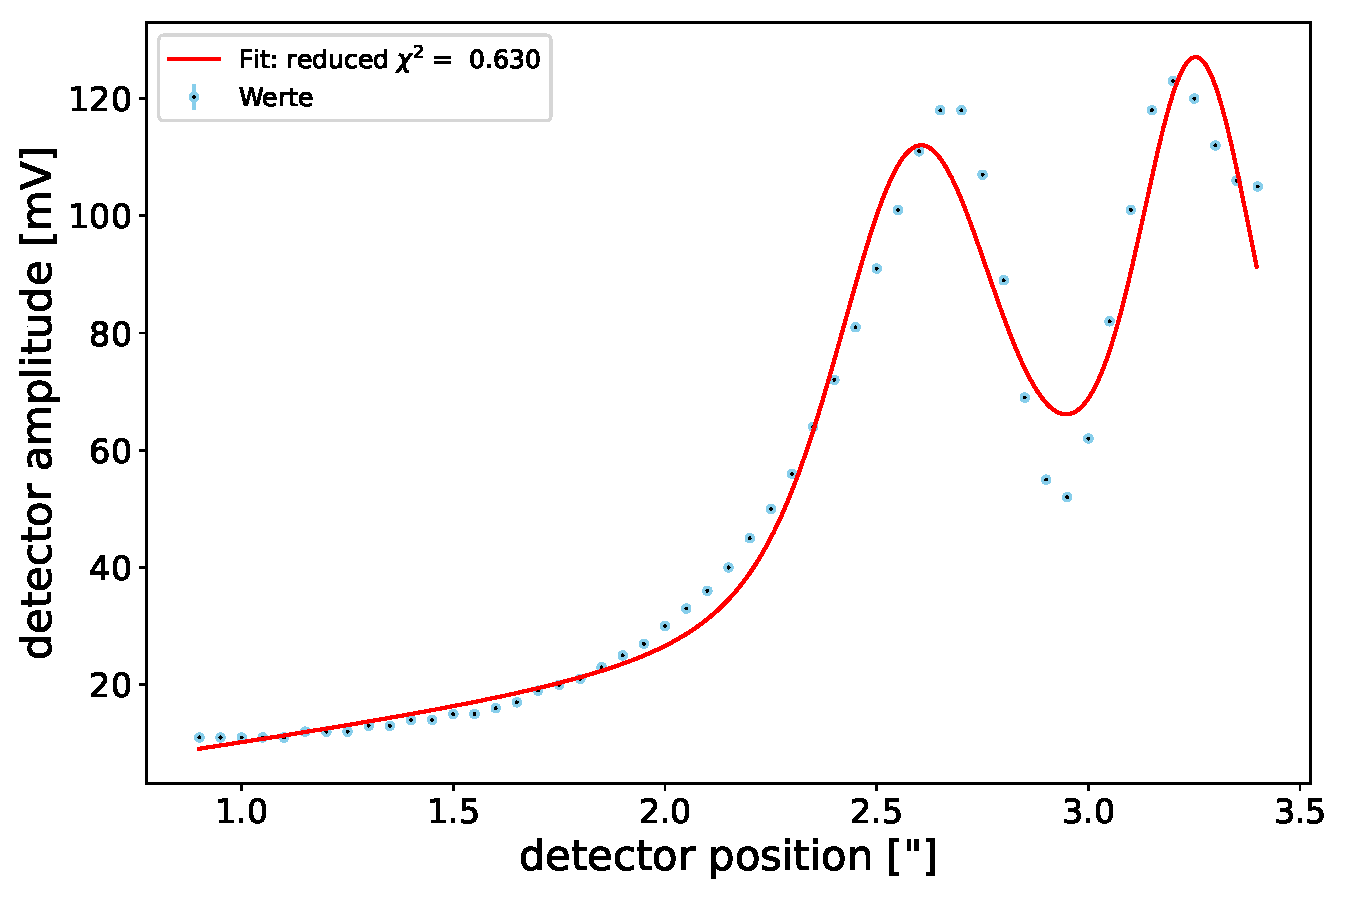
\includegraphics[width= 0.65 \textwidth]{Fits/Amps_B05A1_Fit.pdf} 
	\caption{Amps_B05A1, Fit} 
 	\label{fig:Amps_B05A1, Fit} 
\end{figure}
 \\ 
\begin{table}[ht] 
\centering 
\caption{Amps_B05A, Fit Parameter Tabelle} 
\label{tab:my-table}
\begin{tabular}{|l|c|}
\hline
Parameter Name	&	Wert \\ \hline
aamplitude	&	 52.238 \pm  4.780\\ \hline
acenter	&	 2.597 \pm  0.0106\\ \hline
asigma	&	 0.13 \pm  0.0102\\ \hline
bamplitude	&	 40.967 \pm  4.409\\ \hline
bcenter	&	 3.255 \pm  0.0107\\ \hline
bsigma	&	 0.095 \pm  0.00978\\ \hline
slope	&	 9.999 \pm  2.397\\ \hline
intercept	&	-0.90445 \pm  3.068\\ \hline
agamma	&	 0.13 \pm  0.0102\\ \hline
afwhm	&	 0.468 \pm  0.0367\\ \hline
aheight	&	 83.916 \pm  4.506\\ \hline
bgamma	&	 0.095 \pm  0.00978\\ \hline
bfwhm	&	 0.342 \pm  0.0352\\ \hline
bheight	&	 90.009 \pm  6.521\\ \hline
\end{tabular} 
\end{table}